% ---------------------------------------------------------------
% TEMPLATE TCC2 - SENAC SANTO AMARO
% ---------------------------------------------------------------
% Trabalho de Conclusão de Curso 2
% Elaborado para apresentação do trabalho final do TCC
% Estrutura: Introdução, Revisão Bibliográfica, Metodologia,
%            Desenvolvimento, Resultados e Análise, Conclusão
% ---------------------------------------------------------------

\documentclass[
    12pt,                % tamanho da fonte
    openright,           % capítulos começam em página ímpar
    oneside,             % para impressão em apenas um lado do papel
    a4paper,             % tamanho do papel
    english,             % idioma adicional
    brazil               % idioma principal
]{abntex2}

% ---------------------------------------------------------------
% PACOTES
% ---------------------------------------------------------------
\usepackage{lmodern}                % Fonte Latin Modern
\usepackage[T1]{fontenc}            % Seleção de códigos de fonte
\usepackage[utf8]{inputenc}         % Codificação do documento
\usepackage{lastpage}               % Usado pela Ficha catalográfica
\usepackage{indentfirst}            % Indenta o primeiro parágrafo
\usepackage{color}                  % Controle de cores
\usepackage{graphicx}               % Inclusão de gráficos
\usepackage{microtype}              % Melhorias de justificação
\usepackage{float}                  % Para posicionamento de figuras
\usepackage{booktabs}               % Tabelas profissionais
\usepackage{multirow}               % Células mescladas em tabelas
\usepackage{longtable}              % Tabelas longas
\usepackage{amsmath,amssymb}        % Símbolos matemáticos
\usepackage{pgfgantt}               % Diagramas de Gantt
\usepackage[brazilian,hyperpageref]{backref}  % Páginas com citações
\usepackage[alf]{abntex2cite}       % Citações ABNT
\usepackage{algorithm}
\usepackage{algpseudocode}
\usepackage{minted}

\floatname{algorithm}{Algoritmo}
\renewcommand{\algorithmicrequire}{\textbf{Entrada:}}
\renewcommand{\algorithmicensure}{\textbf{Saída:}}
\renewcommand{\algorithmicfunction}{\textbf{Função}}

% ---------------------------------------------------------------
% CONFIGURAÇÕES DO PDF
% ---------------------------------------------------------------
\makeatletter
\hypersetup{
    pdftitle={\@title},
    pdfauthor={\@author},
    pdfsubject={TCC2 - SENAC Santo Amaro},
    pdfcreator={LaTeX with abnTeX2},
    pdfkeywords={tcc2}{senac}{santo amaro}{trabalho de conclusão},
    colorlinks=true,        % false: links em caixas; true: links coloridos
    linkcolor=blue,         % cor dos links internos
    citecolor=blue,         % cor dos links para bibliografia
    filecolor=magenta,      % cor dos links para arquivos
    urlcolor=blue,
    bookmarksdepth=4
}
\makeatother

% ---------------------------------------------------------------
% CONFIGURAÇÕES DE APARÊNCIA DO PDF FINAL
% ---------------------------------------------------------------
\definecolor{blue}{RGB}{41,5,195}

% ---------------------------------------------------------------
% TAMANHO DA FONTE DAS LEGENDAS (ABNT) -- 10 pt
% ---------------------------------------------------------------
% O título (\caption) e a linha de fonte (\legend) de figuras e
% tabelas devem ficar em 10 pt (o corpo do texto é 12 pt). Por
% padrão o memoir/abntex2 deixa essas legendas em 12 pt; os comandos
% abaixo reduzem o título e a fonte para 10 pt.
\renewcommand{\ABNTEXfontereduzida}{\fontsize{10}{12}\selectfont}
\captionnamefont{\ABNTEXfontereduzida}   % rótulo "Figura N"/"Tabela N"
\captiontitlefont{\ABNTEXfontereduzida}  % texto do título da legenda
\makeatletter
% Redefine \legend (usado em "Fonte: ...") para sair em 10 pt
% (a definição original do memoir fixa \normalsize = 12 pt).
\renewcommand{\legend}[1]{%
  \M@gettitle{#1}%
  \memlegendinfo{#1}%
  \par
  \begingroup
    \@parboxrestore
    \if@minipage
      \@setminipage
    \fi
    \ABNTEXfontereduzida
    \captiondelim{\mbox{}}%
    \@makecaption{}{\ignorespaces #1}\par
  \endgroup}
\makeatother

% ---------------------------------------------------------------
% INFORMAÇÕES DO DOCUMENTO
% ---------------------------------------------------------------
\titulo{Detecção de vulnerabilidades de memória em C: Abordagem integrando VSA e HOFG}
\autor{Lucas Zacarias Martins Neves}
\local{São Paulo}
\data{2026}
\orientador{Prof. Leonardo Massayuki Takuno}
% \coorientador{Prof. Nome do Coorientador} % Descomente se houver coorientador
\instituicao{%
  SENAC -- Serviço Nacional de Aprendizagem Comercial
  \par
  Unidade Santo Amaro
  \par
  Bacharelado em Ciência da computação
}

\tipotrabalho{Trabalho de Conclusão de Curso II}

\preambulo{Trabalho de Conclusão de Curso II apresentado ao SENAC Santo Amaro como requisito parcial para conclusão do curso de Bacharelado em Ciência da computação.}

% ---------------------------------------------------------------
% COMPILA O ÍNDICE
% ---------------------------------------------------------------
\makeindex

% ---------------------------------------------------------------
% INÍCIO DO DOCUMENTO
% ---------------------------------------------------------------
\begin{document}

% Seleciona o idioma do documento
\selectlanguage{brazil}

% Retira espaço extra obsoleto entre as frases
\frenchspacing

% ---------------------------------------------------------------
% ELEMENTOS PRÉ-TEXTUAIS
% ---------------------------------------------------------------
\pretextual

% ---------------------------------------------------------------
% CAPA
% ---------------------------------------------------------------
\imprimircapa

% ---------------------------------------------------------------
% FOLHA DE ROSTO
% ---------------------------------------------------------------
\imprimirfolhaderosto

% ---------------------------------------------------------------
% RESUMO
% ---------------------------------------------------------------
\begin{resumo}

\vspace{\onelineskip}

Vulnerabilidades de segurança de memória em linguagens como C e C++ representam uma parcela significativa das falhas críticas de software na indústria. 
Ferramentas de análise estática são fundamentais para a detecção precoce dessas falhas, mas frequentemente esbarram em limitações, como a alta taxa de falsos positivos. 
O modelo estrutural \textit{Heap Object Flow Graph} (HOFG) destaca-se por rastrear o fluxo de blocos alocados dinamicamente na memória \textit{Heap}; contudo, sua implementação original apresenta dificuldades no tratamento de aritmética de ponteiros, 
resultando em cerca de 14\% de imprecisões em testes preliminares. Para mitigar essa limitação, este trabalho propõe o desenvolvimento de um analisador estático que integra o HOFG com a técnica de interpretação abstrata \textit{Value-Set Analysis} (VSA). 
A ferramenta, construída na linguagem Zig e operando sobre a Representação Intermediária do compilador LLVM (LLVM IR), adota um processamento modular de arquivos para otimizar o consumo de memória RAM. Nessa arquitetura, o VSA atua como um validador numérico sobre o grafo, estimando os limites de deslocamento (\textit{offsets} e \textit{ranges}) 
que cada endereço abstrato pode assumir e impedindo a formação de arestas de fluxo inválidas. A avaliação da precisão e eficiência da solução proposta será conduzida utilizando casos sintéticos do \textit{Juliet Test Suite} e análises de projetos reais de código aberto. O objetivo central é demonstrar que a unificação entre o rastreamento direcional do HOFG e a 
abstração numérica do VSA permite reduzir consideravelmente os falsos positivos na detecção de vulnerabilidades de memória (tais como CWE-401, CWE-415 e CWE-416), garantindo maior segurança e escalabilidade no ciclo de desenvolvimento de software.

\vspace{\onelineskip}

\noindent
\textbf{Palavras-chave}: Análise estática, Vulnerabilidades de memória, HOFG.
\end{resumo}

% ---------------------------------------------------------------
% ABSTRACT (RESUMO EM LÍNGUA ESTRANGEIRA) -- OBRIGATÓRIO NO TCC2
% ---------------------------------------------------------------
% Versão em inglês do resumo. Deve conter o mesmo conteúdo do resumo
% em português (problema, objetivo, método, resultados e conclusão)
% e as palavras-chave traduzidas (Keywords). Pela ABNT NBR 14724, o
% resumo em língua estrangeira vem logo após o resumo em português.
\begin{resumo}[Abstract]
 \begin{otherlanguage*}{english}
   This document presents the undergraduate final project (TCC2) developed at SENAC Santo Amaro, based on the structure recommended by Raul Sidnei Wazlawick in \textit{Metodologia de Pesquisa para Ciência da Computação}. The focus is on highlighting the problem, the objectives, the method, the development, the results and the scientific contribution of the work, avoiding merely descriptive texts. The document is organized into chapters presenting the introduction to the topic, the literature review that grounds the research, the adopted methodology, the development of the solution, the results and their critical analysis, followed by the conclusion and the bibliographic references.

   \vspace{\onelineskip}

   \noindent
   \textbf{Keywords}: keyword1. keyword2. keyword3. keyword4. keyword5.
 \end{otherlanguage*}
\end{resumo}

% ---------------------------------------------------------------
% LISTA DE ILUSTRAÇÕES (FIGURAS)
% ---------------------------------------------------------------
% Gerada automaticamente a partir das \caption{} das figuras.
% Toda figura com legenda passa a constar nesta lista.
\pdfbookmark[0]{\listfigurename}{lof}
\listoffigures*
\cleardoublepage

% ---------------------------------------------------------------
% LISTA DE TABELAS
% ---------------------------------------------------------------
% Gerada automaticamente a partir das \caption{} das tabelas.
% \pdfbookmark[0]{\listtablename}{lot}
% \listoftables*
% \cleardoublepage

% ---------------------------------------------------------------
% LISTA DE ABREVIATURAS E SIGLAS
% ---------------------------------------------------------------
% Esta lista deve vir antes do início do trabalho (elementos pré-textuais).
% Em ordem alfabética, relacione APENAS as abreviaturas e siglas que
% realmente aparecem no texto. Edite a tabela conforme o seu trabalho.
\pdfbookmark[0]{Lista de Abreviaturas e Siglas}{loas}
\chapter*{Lista de Abreviaturas e Siglas}

\noindent A lista a seguir reúne, em ordem alfabética, as abreviaturas e siglas utilizadas neste trabalho, acompanhadas de seus respectivos significados. Substitua, acrescente ou remova linhas conforme a necessidade do seu projeto.

\vspace{\onelineskip}

\begin{center}
\begin{tabular}{@{}p{3.2cm}p{0.6\textwidth}@{}}
\toprule
\textbf{Abreviatura} & \textbf{Significado} \\
\midrule
AST & \textit{Abstract Syntax Tree} (Árvore sintática abstrata) \\
CFG & \textit{Control Flow Graph} (Grafo de fluxo de controle) \\
CVE & \textit{Common Vulnerabilities and Exposures} \\
CVSS & \textit{Common Vulnerability Scoring System} \\
CWE & \textit{Common Weakness Enumeration} \\
HOFG & \textit{Heap Object Flow Graph} \\
IR & \textit{Intermediate Representation} (Representação intermediária) \\
LoC & \textit{Lines of Code} (Linhas de código) \\
MAD & \textit{Memory allocation/deallocation} (Alocação e desalocação de memória) \\
MSRC & \textit{Microsoft Security Response Center} \\
NVD & \textit{National Vulnerability Database} \\
SSA & \textit{Static Single Assignment} (Atribuição única estática)\\
VSA & \textit{Value-Set Analysis} \\
\bottomrule
\end{tabular}
\end{center}

\cleardoublepage


% ---------------------------------------------------------------
% SUMÁRIO
% ---------------------------------------------------------------
\pdfbookmark[0]{\contentsname}{toc}
\tableofcontents*
\cleardoublepage

% ---------------------------------------------------------------
% ELEMENTOS TEXTUAIS
% ---------------------------------------------------------------
\textual

% ===============================================================
% CAPÍTULO 1 - INTRODUÇÃO
% ===============================================================
\chapter{Introdução}
\label{cap:introducao}

Este capítulo introdutório está estruturado nas subseções \ref{sec:Contexto} Contexto, \ref{sec:Justificativa} Justificativa, \ref{sec:Hipotese} Hipótese e \ref{sec:Objetivos} Objetivos, abrangendo objetivo geral e objetivos específicos.


\section{Contexto}
\label{sec:Contexto}

Em um levantamento realizado pela \textit{Microsoft Security Response Center} (MSRC) realizado em 2019 \cite{MSRC2019},
foi apurado que aproximadamente 70\% das vulnerabilidades corrigidas em softwares da multinacional entre o período de 2004 e 2018 
tem ligação a falhas de segurança de memória nas linguagens C e C++, causadas por desenvolvedores que inseriram tais erros em seus códigos
sem perceber. Além disso, a situação teve piora não somente com o incremento da base de código da empresa, mas também com a adição de mais 
código aberto aos seus projetos.
\par
É pontuado ainda pela Microsoft que existem métodos para auxiliar os desenvolvedores a desenvolver código seguro, 
tais métodos variam desde ferramentas e algoritmos desenvolvidos para análise do próprio código escrito até a guias e metodologias de desenvolvimento para software seguro, 
treinamentos internos, reuniões para monitoria e análise de código. Salvaguardas que atuam em todas as camadas do desenvolvimento de software, 
e mesmo com tais itens, tais vulnerabilidades de memória continuam predominantes.
\par
Dando destaque às ferramentas de análise de código estático, por vezes exigem tempo para que os desenvolvedores aprendam a fazer uso do analisador, 
cenário este que torna o uso de tais ferramentas algo inviável quando o tempo não é aliado. Além disso, tais ferramentas não garantem que todas 
as vulnerabilidades e possíveis falhas de um código sejam encontradas, pois focam numa análise do código-fonte do software, sendo escrito numa linguagem de alto nível e 
não na linguagem de máquina gerada pelo compilador que será executada pelo hardware \cite{Balakrishnan2010}.
\par
Além de métodos de código estático, outra opção também pontuada pela MSRC para a diminuição de ocorrências, seria o uso de linguagens de programação \textit{memory-safe}, ou seja,
que retiram das mãos de desenvolvedores os ônus de preocupações com segurança de memória e a adicionam na própria linguagem, 
fazendo gerenciamento de memória ou empregando regras estritas na fase de compilação, evitando tais vulnerabilidades.
Um exemplo de linguagem de programação \textit{memory-safe} é o Rust, sendo desenvolvido pela Mozilla e que tem como um de seus princípios a segurança de memória.

\section{Justificativa}
\label{sec:Justificativa}

Apesar da existência de linguagens de programação que integram mecanismos designados para o gerenciamento da memória \textit{Heap}, tais como o C\# e Java, 
e até mesmo com a existência de linguagens de programação que tem como objetivo principal a segurança e estabilidade do programa, como ocorre com o Rust \cite{MSRC2019}, 
a reescrita de projetos inteiros frequentemente apresenta custos excessivos de portabilidade. Diante disso, a manutenção e o desenvolvimento na linguagem original se tornam necessários, 
cenário este que pode ocorrer em projetos construídos em linguagens de programação inseguras, como C e C++.
\par
Para garantir maior segurança de tais projetos, um analisador de código pode ser desenvolvido como solução, com foco na detecção de potenciais vazamentos e 
problemas derivados da má gestão de dados alocados dinamicamente. Embora a análise estática de códigos-fonte apresente limitações — dentre elas, as limitações apresentadas por \citeonline{Balakrishnan2007} —, 
tais abordagens continuam sendo úteis no ciclo de desenvolvimento de software, havendo como uma de suas principais justificativas para adoção a possibilidade de identificar e mitigar vulnerabilidades 
ainda nas fases iniciais do projeto \cite{spa}. 
\par
Além disso, embora possam ocorrer mudanças no código-fonte originadas em tempo de compilação para arquiteturas específicas, havendo ainda a possibilidade de falhas geradas pelo próprio compilador, 
a grande maioria das vulnerabilidades relacionadas à segurança de memória são geradas pelos próprios desenvolvedores de forma desavisada \cite{MSRC2019}, permanecendo no código-fonte e passíveis de detecção 
através de algoritmos.


\section{Hipótese}
\label{sec:Hipotese}

A hipótese do projeto está numa integração entre dois métodos de análise estática. 
\par
O primeiro método é o \textit{Heap Object Flow Graph} (HOFG) \cite{MadhavC2023}, sendo uma representação do fluxo dos blocos de memória alocados na \textit{Heap}, na qual os vértices do grafo são obtidos 
a partir das variáveis do programa que são ponteiros para a memória \textit{Heap}.
\par
Para automatizar a detecção de vulnerabilidades de memória, foi desenvolvido o \textit{HOFG-Analyser}, uma ferramenta de análise estática que utiliza a representação HOFG para a detecção de tais vulnerabilidades. 
O processo tem início com a compilação do código-fonte por meio da infraestrutura do \textit{framework} LLVM, com objetivo de gerar a representação intermediária (LLVM IR) da aplicação. A partir dessa versão estruturada na IR, 
o grafo de fluxo de objetos na memória \textit{Heap} é construído, abrangendo o programa completo. Após a geração completa do grafo, o \textit{HOFG-Analyser} realiza as verificações necessárias a procura de potenciais vazamentos ou falhas de memória \cite{MadhavC2023}.
\par 
Porém, o \textit{HOFG-Analyser} obteve 14\% de falsos positivos em seus testes, apresentando dificuldades com aritmética de ponteiros presente na linguagem C, ocorrendo pois, dado um ponteiro $p$, as operações $q = p + 1$ e $q = p$ resultam na adição de uma mesma aresta do 
ponteiro $p$ para o ponteiro $q$ no grafo. Como consequência, as instruções $free(p)$ e $free(q)$ seriam interpretadas de forma simplificada como a liberação do mesmo objeto na memória \textit{Heap} \cite{MadhavC2023}.
\par
Para lidar com as dificuldades presentes pela aritmética de ponteiros e ser possível diminuir a taxa de falsos positivos do HOFG original, 
uma integração com o \textit{Value-Set Analysis} (VSA) \cite{Balakrishnan2007} poderia ser realizada. O VSA, técnica de interpretação abstrata originalmente aplicada para análise de executáveis, 
tem o objetivo de encontrar uma aproximação segura para o conjunto de valores que cada objeto de dados pode armazenar em cada ponto de um programa. 
\par
Ao integrar o VSA ao HOFG, o mapeamento dos limites de intervalos de endereços abstratos na memória \textit{Heap} se torna possível, reduzindo a taxa de falsos positivos na detecção de vulnerabilidades comparado a análise baseada unicamente ao modelo HOFG padrão.


\section{Objetivos}
\label{sec:Objetivos}

Os objetivos deste trabalho dividem-se em um objetivo principal e objetivos secundários, os quais representam passos necessários para que o propósito central seja alcançado.

\subsection{Objetivo geral}
\label{sec:Objetivo_geral}

O objetivo principal do trabalho é demonstrar a viabilidade da integração da representação \textit{Heap Object Flow Graph} (HOFG) com técnicas de \textit{Value-Set Analysis} (VSA) para o rastreamento preciso de ponteiros (\textit{offset} e \textit{range}), com foco na detecção de vulnerabilidades de memória em análise estática de código para a linguagem C.

\subsection{Objetivos específicos}
\label{sec:Objetivos_especificos}

\begin{enumerate}
    \item Fundamentar teoricamente a integração do \textit{Value-Set analysis} à estrutura do \textit{Heap Object Flow Graph} (HOFG), demonstrando como essa abordagem conjunta pode mitigar as limitações de rastreamento de ponteiros e reduzir a taxa de falsos positivos da análise estática.
    \item Implementar motor de análise estática processando a representação intermediária LLVM IR, construindo os algoritmos necessários para a extração e geração do HOFG e sua integração com o VSA.
    \item Avaliar a precisão e a eficiência do analisador implementado utilizando conjuntos de testes que exploram falhas da linguagem C (como vazamentos de memória e usos após desalocação). 
    \item Comparar os resultados obtidos com referências comparativas tendo como foco principal a taxa de falsos positivos e verdadeiro positivos, e comparar o tempo e custo computacional da implementação original do HOFG, para validar o impacto da integração.
\end{enumerate}


% ===============================================================
% CAPÍTULO 2 - REVISÃO BIBLIOGRÁFICA / TRABALHOS RELACIONADOS
% ===============================================================

\chapter{Revisão Bibliográfica}
\label{cap:revisao}

A revisão bibliográfica deste artigo está estruturada nas subseções \ref{sec:metodologia_pesquisa} Metodologia da pesquisa bibliográfica, abrangendo a forma como a pesquisa bibliográfica foi conduzida; 
\ref{sec:referencial} Referencial, contendo os principais conceitos, teorias e definições que constituem a base fundamental deste trabalho; \ref{sec:metricas_de_avaliacao} Métricas de avaliação, detalhando como a solução proposta será avaliada e o que será levado em consideração; 
e, por fim, \ref{sec:trabalhos_relacionados} Trabalhos relacionados, subseção que contém breve análise de três artigos com objetivos similares, destacando suas características, resultados obtidos e, principalmente, as distinções em relação a este trabalho.


% ---------------------------------------------------------------
\section{Metodologia da pesquisa bibliográfica}
\label{sec:metodologia_pesquisa}

\par
A pesquisa bibliográfica foi realizada primariamente no motor de busca Google Acadêmico (\textit{Google Scholar}), utilizando as seguintes strings de busca:

\begin{itemize}
\item \textit{"memory leak" AND "static analysis"}
\item \textit{"memory leak" AND "dynamic analysis"}
\item \textit{("memory safety" OR "memory leak" OR "memory corruption") AND ("empirical study" OR "quantitative analysis") AND "vulnerability"}
\end{itemize}

\par
A exclusão de artigos foi guiada por critérios de inclusão e exclusão predefinidos. Foram considerados trabalhos publicados no período entre 2022 e 2026, primariamente em língua inglesa e que abordassem diretamente métodos de identificação de vulnerabilidades de memória.

\par
Após a busca inicial, técnica de triagem (\textit{screening}) foi empregada, consistindo na avaliação do título e do resumo de cada artigo obtido. Essa etapa resultou na seleção de 11 artigos, focados em métodos de análise para detecção dessas vulnerabilidades. 
Dentre estes, o trabalho seminal referente ao modelo \textit{Heap Object Flow Graph} (HOFG) ganhou destaque por ter como foco a adaptação da estrutura para a detecção de vulnerabilidades de memória na linguagem C.

\par 
Em seguida, foram mapeados os trabalhos seminais referenciadas pelos autores. Essa etapa de pesquisa em cadeia (\textit{snowballing}), totalizando 24 artigos. Contudo, com o modelo HOFG estabelecido como base estrutural, a etapa de leitura recebeu um filtro de exclusão mais restrito, sendo considerados e lidos artigos com ligação direta a base estrutural.

\par
Por fim, a partir de necessidades conceituais levantadas durante a leitura de tais artigos, busca complementar foi conduzida, utilizando como referência a literatura clássica, livros técnicos e documentações oficiais com o objetivo de obter definições estruturais necessárias.
% ---------------------------------------------------------------


\section{Referencial}
\label{sec:referencial}

Para fundamentar o desenvolvimento do analisador proposto, esta seção estabelece os alicerces teóricos da pesquisa. O texto está estruturado a partir dos conceitos de Memória \textit{Heap} (\ref{subsec:HEAP}) e Análise Estática (\ref{subsec:analise_estatica}), 
avançando para a infraestrutura de compilação LLVM (\ref{subsec:llvm}), e a classificação de Vulnerabilidades de Memória (\ref{subsec:vulnerabilidades_memoria}). Por fim, são detalhados os dois modelos centrais que embasam a solução: \textit{Heap Object Flow Graph} (\ref{subsec:HOFG}) e \textit{Value-Set Analysis} (\ref{subsec:VSA}).

\subsection{Memória \textit{Heap}}
\label{subsec:HEAP}

A memória \textit{Heap} é uma área da memória virtual de um processo utilizada para a alocação dinâmica de memória. Tal região tem início logo após a área de dados não inicializados do programa e cresce para cima, 
em direção a endereços de memória mais altos. Para cada processo, o \textit{kernel} mantém uma variável brk (sendo pronunciada \textit{break}, ou quebra) que aponta para o topo da \textit{Heap} \cite{Bryant2010}. 
Um alocador dinâmico gerencia a \textit{Heap} como uma coleção de blocos de tamanhos variados. Cada bloco é um segmento (\textit{chunk}) contínuo de memória virtual que pode estar em dois estados: alocado ou livre. 
Um bloco alocado é reservado para uso de forma explícita pela aplicação, permanecendo neste estado até que seja liberado, tanto de forma explícita, pelo aplicativo, quanto de forma implícita, pelo próprio alocador de memória (como em sistemas com \textit{Garbage Collection}). 
E, por sua vez, um bloco livre está disponível para ser alocado, e permanece assim até que, de forma explícita, seja alocado através de uma nova requisição de alocação feita pela aplicação. O fato de que, por vezes, o tamanho exato de certas estruturas de dados que 
serão utilizados em um programa só se tornam conhecidos até que o mesmo seja executado se torna o principal motivo para a utilização da alocação dinâmica de memória e, consequentemente, da memória \textit{Heap} \cite{Bryant2010}.


\begin{figure}[htpb]
\centering
\caption{Função em C utilizada como base para as representações intermediárias.}
\label{fig:codigo_exemplo}
\begin{minted}[linenos, frame=single, fontsize=\small]{c}
int exemplo() {

    int i = 0;
    int v = 10;

    do { 
        if (i % 2 == 0) {
            i = i + 1;
        }
        else {
            i = i * 2;
        }
    } while (i < v);

    return i;
}
\end{minted}
\legend{Fonte: Elaborado pelo autor (2026)}
\end{figure}

\subsection{Análise estática}
\label{subsec:analise_estatica}

\par
A análise estática de programas é definida como a arte de raciocinar sobre o comportamento de programas sem de fato executá-los. O seu objetivo principal é responder de forma automatizada perguntas sobre os possíveis comportamentos de um código. 
Isto é útil não apenas em otimizações realizadas por um compilador para produzir código binário eficiente, mas também para detecção automatizada de erros e outras ferramentas que podem ajudar programadores. Um analisador estático de programas é um programa que faz inferências sobre o comportamento de outros programas \cite{spa}.

O código-fonte escrito em C apresentado na figura \ref{fig:codigo_exemplo} servirá como exemplo para ilustrar as transformações abordadas nesta seção. Serão obtidas as suas representações
intermediárias: a Árvore sintática abstrata (AST), o Grafo de fluxo de controle (CFG) e, por fim, a forma de Atribuição Única Estática (SSA).

\subsubsection{Árvore sintática abstrata (AST)}

\begin{figure}[htpb]
\centering
\caption{Código presente na figura \ref{fig:codigo_exemplo} na forma AST de baixa fidelidade}
\label{fig:codigo_cfg}
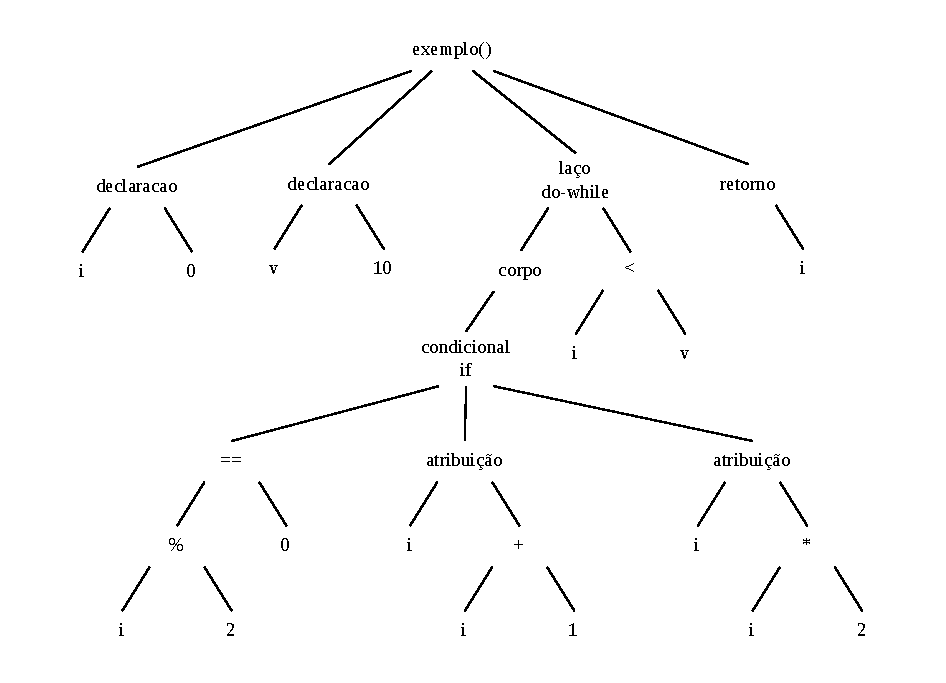
\includegraphics[width=\textwidth]{ast_exemplo.pdf}
\legend{Fonte: Elaborado pelo autor (2026)}
\end{figure}


Segundo \citeonline{Compilers2009}, as árvores sintáticas abstratas (ASTs), ou simplesmente árvores sintáticas, nas quais cada nó interno representa um operador da expressão, e seus nós filhos representam os respectivos operandos.
Além disso, as ASTs se assemelham às árvores de derivação até certo nível, diferenciando-se pelo fato de que os nós interiores da AST representam construções de programação, ao passo que na árvore de derivação os nós 
interiores representam símbolos não-terminais. Outra diferença é a ausência de símbolos não-terminais auxiliares, tais como aqueles que representam termos, fatores, ou outras variações de expressões, na AST. 
Essa falta ocorre pois tais detalhes sintáticos são desnecessários para a fase de tradução, resultando em uma representação mais condensada e focada na semântica do código-fonte.

\par
A figura \ref{fig:codigo_cfg} ilustra a representação AST da função exemplo exibida na figura \ref{fig:codigo_exemplo}. Por ser uma representação de baixa fidelidade, a árvore foca na estrutura lógica das operações, abstraindo a pontuação original do código-fonte. 
A raiz ramifica-se sequencialmente para as operações principais: as declarações das variáveis \texttt{i} e \texttt{v}, a estrutura de repetição \texttt{do-while}, declarando seu corpo e a sua condição de parada \texttt{<}, e, por fim, o nó de retorno da função.

\subsubsection{Grafo de fluxo de controle (CFG)}

\begin{figure}[htpb]
\centering
\caption{Código presente na figura \ref{fig:codigo_exemplo} em sua forma CFG}
\label{fig:codigo_cfg}
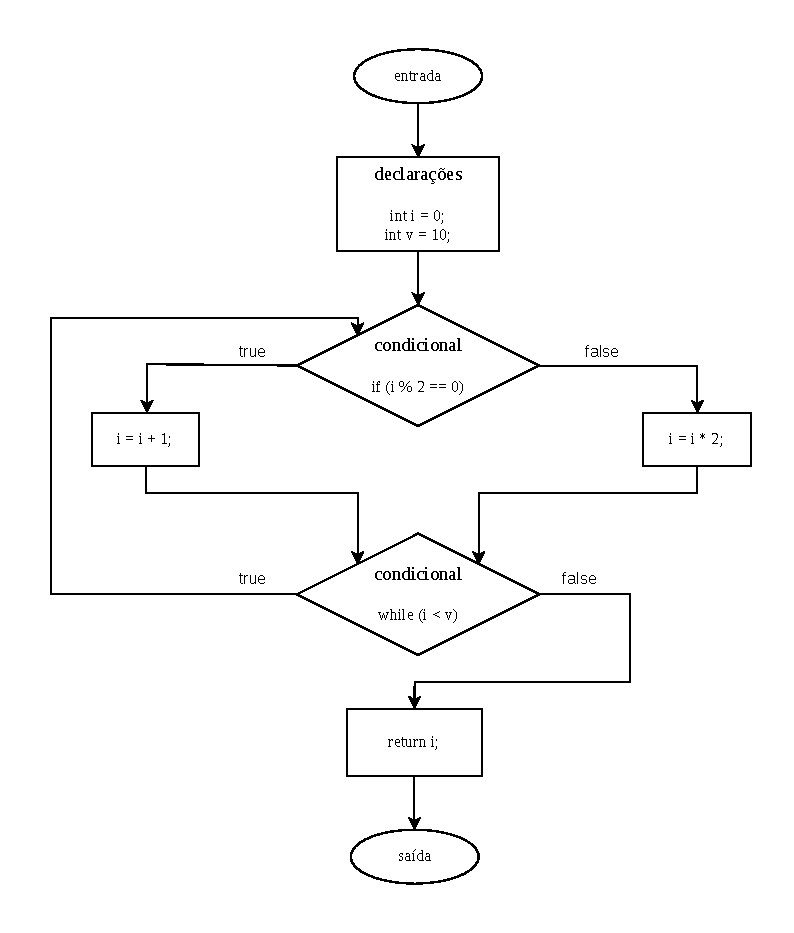
\includegraphics[width=0.8\textwidth]{cfg_exemplo.pdf}
\legend{Fonte: Elaborado pelo autor (2026)}
\end{figure}

Um grafo de fluxo de controle (\textit{Control Flow Graph}, ou CFG) é um grafo direcionado, no qual seus vértices correspondem a declarações (instruções) e arestas representam possíveis caminhos do fluxo de controle durante a execução. Para simplificar as representações e algoritmos que operam sobre o grafo, 
é assumido por convenção que todo CFG possui um único ponto de entrada ($entry$) e um único ponto de saída ($exit$), os quais podem ser compreendidos como comandos vazios (\textit{no-ops}). Além disso, se $v$ é um vértice presente em um CFG, então $pred(v)$ denota o conjunto de vértices predecessores e $succ(v)$ o conjunto de vértices sucessores. 
Para programas totalmente normalizados, cada vértice corresponde a apenas uma operação \cite{spa}. 

\par
O emprego de um CFG se dá pelo fornecimento de uma representação de código que mantém a ordem em que as instruções são executadas, criando contraste com ASTs, que representam a estrutura sintática do programa enquanto ignoram a ordem de execução dos comandos. Por fornecer tal ordem de execução de instruções, 
o CFG se torna adequado para análises sensíveis ao fluxo (\textit{flow-sensitive analysis}), especialmente a análise de fluxo de dados (\textit{dataflow analysis}) \cite{spa}.

\par
Os CFGs podem ser construídos de maneira indutiva para as diferentes estruturas de uma linguagem. Comandos em sequência são unidos, eliminando a saída do primeiro e a entrada do segundo, bem como estruturas de decisão (\textit{if-else}) e laços de repetição (\textit{while}) dividem o fluxo em arestas de ramificação, 
comumente rotuladas com as condições verdadeiro ou falso \cite{spa}.

\par
A figura \ref{fig:codigo_cfg} apresenta o CFG correspondente à execução da função \texttt{exemplo}, presente na figura \ref{fig:codigo_exemplo}. A partir do nó de entrada, o fluxo sequencial passa pelas declarações iniciais até atingir a condicional \texttt{if(i \% 2 == 0)}. 
As arestas direcionadas ilustram as duas ramificações mutuamente exclusivas que convergem para a avaliação do laço \texttt{while (i < v)}. Uma aresta de retorno demonstra o ciclo do laço quando a condição é mantida como verdadeira, ao passo que o caminho alternativo conduz à instrução de retorno e ao término da função.

\subsubsection{Níveis de sensibilidade da análise estática}

Os níveis de sensibilidade são características que definem como uma ferramenta de análise estática modela e percorre o código-fonte. No que diz respeito à ordem de execução, as análises podem ser categorizadas em duas abordagens principais \cite{spa}:

\par
\textbf{Análise sensível ao fluxo}, (\textit{Flow-Sensitive}): Abordagem que leva em consideração a ordem em que as instruções de um programa são executadas, a partir disso, se torna capaz de distinguir entre os diferentes pontos de um programa. 
Por exemplo, se uma variável $a$ recebe uma atribuição na linha $2$ e outra atribuição na linha $4$, a análise sensível ao fluxo é capaz de reconhecer que uma leitura realizada na linha $3$ dependerá estritamente do valor definido na linha $2$, e não da linha $4$ \cite{spa}.

\par
\textbf{Análise insensível ao fluxo}, (\textit{Flow-Insensitive}): Abordagem que ignora a ordem de execução das instruções de um programa. Tal análise enxerga o código como um conjunto não ordenado de comandos. Por conta disso, tais análises frequentemente utilizam ASTs como representação base, 
já que tal estrutura capta a sintaxe global do programa, sem haver preocupação com o sequenciamento temporal do fluxo. Seu uso esta em métodos que não dependem da cronologia de um programa para realizar sua análise, tais como a análise de tipos \cite{spa}.


\subsubsection{Forma de atribuição única estática (SSA)}

\begin{figure}[htpb]
\centering
\caption{Código presente na figura \ref{fig:codigo_exemplo} adaptado para a forma SSA de forma didática}
\label{fig:codigo_ssa}
\begin{minted}[linenos, frame=single, fontsize=\small]{c}
int exemplo() {
    i1 = 0;
    v1 = 10;

    do {
        i2 = phi(i1, i5); 

        if (i2 % 2 == 0) {
            i3 = i2 + 1;
        } 
        else {
            i4 = i2 * 2;
        }

        i5 = phi(i3, i4);

    } while (i5 < v1);

    return i5;
}
\end{minted}
\legend{Fonte: Elaborado pelo autor (2026)}
\end{figure}


O SSA (\textit{Static Single Assignment}) é uma forma de representação de código intermediário, tem como ponto-chave as características de que cada definição de variável possui um nome distinto, e de que cada uso refere-se a apenas uma única definição, 
sendo essas também as duas restrições da representação, significando que, caso um programa atenda tais restrições, tal programa estará em sua forma SSA. Para garantir essa singularidade, variáveis que sofrem múltiplas atribuições no código-fonte são renomeadas, 
sendo criadas versões distintas para cada nova atribuição (por exemplo, $v1$, $v2$, $v3$) \cite{Singer2022}. 

\par
Além disso, em programas com desvios do fluxo de controle, contendo blocos condicionais e laços de repetição, diferentes versões da mesma variável podem chegar ao mesmo ponto de convergência no 
Grafo de Fluxo de Controle (CFG). São inseridas então, nesses pontos de junção, as chamadas funções $\phi$ (\textit{phi functions}), possuindo $N$ argumentos correspondentes aos $N$ caminhos do fluxo de controle convergentes, 
e seleciona a versão correta da variável com base no caminho de execução tomado pelo programa. Sendo criada inicialmente para facilitar o desenvolvimento de transformações de programa de alto nível, 
a forma ganhou popularidade pelas suas propriedades que permitem a simplificação de algoritmos e a redução da complexidade computacional das análises de fluxo de dados. Atualmente, 
é amplamente utilizada por compiladores de código aberto e comerciais, como é o caso do LLVM, sendo uma estrutura fundamental para a análise estática de programas \cite{Singer2022}.

\par
O trecho de código, presente na figura \ref{fig:codigo_ssa}, ilustra uma adaptação didática da função exemplo presente na figura \ref{fig:codigo_exemplo} para a forma SSA. Para satisfazer as propriedades da representação SSA, a variável original \texttt{i} é 
versionada em múltiplas instâncias independentes. Além disso, o código exibe o uso de funções $\phi$ em dois pontos de convergência do fluxo: no início do laço \texttt{do-while}, para mesclar o valor inicial da variável com o valor propagado pela iteração anterior (\texttt{i2 = phi(i1, i5)}), 
e logo após a condicional \texttt{if-else}, para unificar as ramificações exclusivas da execução (\texttt{i5 = phi(i3, i4)}) antes da verificação para continuidade do laço.

\subsubsection{Limitações da análise estática em códigos-fonte}

Os métodos de análise estática não garantem que todas as vulnerabilidades de um código-fonte sejam encontradas. Dentre os motivos, sendo listados por \citeonline{Balakrishnan2007}, estão:

\begin{itemize}
\item 
O uso de bibliotecas já compiladas (tais como as DLLs) em programas, por vezes sem estar disponíveis em sua forma fonte. Gerando a necessidade de realizar esboços 
que simulam os efeitos das chamadas de função de tais bibliotecas. Por não poder realizar a análise em tais bibliotecas, é possível que a mesma possua erros, não sendo detectados durante a 
análise estática sendo realizada, resultando em inconsistências.
\item
O fato de que códigos-fonte são modificados pelo compilador durante a compilação, realizando otimizações e adicionando instrumentações de código, sendo itens não encontrados pelas 
ferramentas que analisam tais códigos.
\item 
O código-fonte de um programa pode ser escrito em mais de uma linguagem de programação, tornando mais dificultoso o design de tais ferramentas de análise, pois precisam dar suporte a 
múltiplas linguagens de programação, cada uma contendo suas características e peculiaridades.
\item
E, mesmo em um código-fonte escrito em apenas uma linguagem de programação de alto nível, tal código pode conter código escrito em \textit{assembly} em certos locais. 
Ferramentas de análise estática normalmente ignoram o código \textit{assembly} adicionado, ou não levam a análise além do código \textit{assembly} adicionado.
\end{itemize}

\subsubsection{Relevância da análise estática em códigos-fonte}

Mesmo com as limitações presentes nos métodos de análise estática de códigos-fonte — dentre elas, as citadas por \citeonline{Balakrishnan2007} —, tais abordagens continuam sendo úteis no ciclo de  desenvolvimento de software. 
Um dos principais motivos para sua adoção é o fato de que tais métodos permitem que vulnerabilidades sejam encontradas ainda nas fases iniciais do projeto, viabilizando a correção prévia e evitando custos elevados nas etapas finais ou em produção \cite{spa}.
\par
Além disso, apesar do código-fonte ser modificado em tempo de compilação através das otimizações e instrumentações e existindo a possibilidade de erros gerados pelo compilador para arquiteturas específicas, a maioria das falhas reside no código original. 
Sendo apontado pela Microsoft, na qual 70\% das falhas corrigidas vinculadas a um CVE em seus softwares tinham como origem vulnerabilidades de memória geradas pelos próprios desenvolvedores, estando presentes e detectáveis em seus respectivos códigos-fonte \cite{MSRC2019}.
\par
Por fim, quanto ao uso de bibliotecas pré-compiladas, bem como a mescla de múltiplas linguagens de programação e trechos escritos em linguagem \textit{assembly}, os métodos de análise estática costumam adotar abordagens conservadoras (isto é, seguras). Ao serem encontrados, 
tais chamadas para funções e trechos inalcançáveis geram alertas durante a análise, lidando com o desconhecido como se pertencesse ao pior cenário possível. Embora essa característica gere falsos positivos durante a avaliação, é cumprido o propósito de evitar falsos negativos. 
Garantindo, dessa forma, que nenhum ponto cabível de vulnerabilidade passe despercebido e que erros reais sejam tratados \cite{spa}.

\subsection{LLVM}
\label{subsec:llvm}

Segundo \citeonline{Lattner2004}, o LLVM é uma infraestrutura de compilação designada para prover transparência e análise e transformação de programas de forma persistente 
durante todo o seu ciclo de vida. O sistema é fundamentado em uma representação intermediária (IR) de baixo nível, baseada na sua forma SSA, permitindo uma ponte universal entre diferentes linguagens 
e arquiteturas. A arquitetura introduz recursos fundamentais para a análise de código:

\begin{itemize}
\item
Um simples sistema de tipagem independente de linguagem que expõe os tipos primitivos usados comumente para implementar atributos de linguagens de alto nível.
\item 
Instrução para endereçamento aritmético, sendo diferente do C puro, o LLVM utiliza uma instrução específica para cálculos de ponteiros que preserva informações de tipo e limites de estruturas, sendo essencial para detectar acessos inválidos.
\item
Mecanismo uniforme de exceções, utilizado para implementar recursos de tratamento de exceções comumente encontrados em linguagens de alto nível de forma eficiente. 
\end{itemize}

\subsubsection{Implementação do Design de três fases}
\label{subsec:design_tres_fases}

Num compilador moderno, três componentes principais são aplicados \cite{Lattner2011}, sendo eles:

\begin{itemize}
\item
O \textit{front end}, responsável por analisar o código-fonte, checar erros e construir a AST específica para a linguagem em questão.
\item
O otimizador, responsável por realizar transformações de código numa tentativa de melhorar o tempo de execução do código, realizando, por exemplo, remoções de itens redundantes que seriam computados.
\item
O \textit{back end}, também conhecido como o gerador de código. Responsável por mapear o código para o conjunto de instruções da arquitetura alvo. Dentre os itens comumente encontrados no back end, estão inclusos a seleção de instruções, alocação de registradores e o escalonamento de instruções.
\end{itemize}

\par 
Com tal padrão a portabilidade de um compilador para uma nova linguagem de programação fonte gera a necessidade de implementação do novo \textit{front end}, mas permitindo que o otimizador e o \textit{back end} sejam reutilizados. 
Porém, esse benefício não fora alcançado em todos os casos já que implementações do padrão de três fases, numa época em que o LLVM estava tendo seu início, em linguagens como Perl, Python, Ruby e Java não 
compartilhavam código entre si, ou seja, cada uma destas linguagens possuía sua própria implementação de \textit{front end}, otimizador e \textit{back end} \cite{Lattner2011}.

\subsubsection{Representação Intermediária (LLVM IR)}
\label{subsec:llvm_ir}

A representação intermediária é o aspecto principal do LLVM, sendo a forma que compilador utiliza para representar o código-fonte sendo compilado. É designada para análises de nível intermediário e 
transformações que são encontradas no setor de otimização de um compilador. Desenhada com objetivos de adicionar suporte para otimizações em tempo de execução não custosas, otimizações interprocedurais, 
análise completa do programa, transformações abrangendo nível de reestruturação, dentre outros, tem como aspecto mais importante o fato de ser definida como uma linguagem de primeira classe com semântica bem definida, 
tendo seu conjunto de instruções próximo do padrão RISC e possuindo como um de seus pilares a forma SSA \cite{Lattner2011}.
\par 
Sendo a única interface para o otimizador do LLVM, se torna o único requisito para escrever um \textit{front end} para a infraestrutura. Por possuir uma forma textual legível, desenvolver um front end que tem como saída 
a representação intermediária do LLVM se torna algo possível e viável. Tal característica é um dos principais fatores para a disseminação da infraestrutura do LLVM em diferentes aplicações, 
já que a completude presente na representação permite que o suporte de uma nova linguagem seja simplificado \cite{Lattner2011}.

\subsection{Vulnerabilidades de memória}
\label{subsec:vulnerabilidades_memoria}

Uma vulnerabilidade, segundo a CVE, é uma ou mais instâncias de fraquezas em um produto que podem ser exploradas, causando impactos negativos na confidencialidade, integridade e disponibilidade do produto, 
um conjunto de condições ou comportamentos que permitem a violação de políticas de segurança implícitas ou explícitas.

\par
No contexto do desenvolvimento de software e análise de código, as vulnerabilidades de memória consistem em falhas no gerenciamento de espaço de endereçamento de um programa. Para o escopo deste trabalho, 
a análise concentra-se especificamente nas instâncias de fraquezas que afetam os dados alocados dinamicamente na memória \textit{Heap}. Na literatura, essas anomalias - que frequentemente envolvem o controle inadequado de ponteiros - são comumente 
referidas como ``corrupção de memória`` ou ``vazamentos de memória``. No entanto, o termo mais abrangente ``vulnerabilidades de memória`` foi escolhido para utilização para evitar ambiguidades com classificações específicas, como a CWE-401 (\textit{Memory Leak}), 
uma vez que o analisador proposto visa englobar anomalias que afetam a memória dinâmica.

\par
Segundo o \textit{Microsoft Security Response Center} (MSRC) \cite{MSRC2019}, entre o período de 2004 a 2018 aproximadamente 70\% das vulnerabilidades corrigidas mapeadas a um CVE foram causadas por desenvolvedores 
que de forma desavisada adicionaram problemas relacionados a vulnerabilidades de memória em seus códigos escritos nas linguagens C e C++. Além disso, a medida que a base de código da Microsoft era incrementada e 
mais código aberto era utilizado, tal problema continuava a aumentar.

\subsubsection{\textit{Common Weakness Enumeration} (CWE)}
\label{subsec:cwe}

A \textit{Common Weakness Enumeration} (CWE) consiste em uma lista desenvolvida de forma colaborativa, que relaciona fraquezas recorrentes em software e hardware. No contexto de segurança, 
uma fraqueza (\textit{weakness}) é uma condição num software, firmware, hardware, ou serviço que, a partir de certas circunstâncias, pode contribuir para a introdução de vulnerabilidades. Fraquezas são identificadas, 
classificadas, descritas e integradas à lista oficial da CWE (\textit{CWE List}). A compreensão dessas fraquezas que resultam em vulnerabilidades permite que desenvolvedores de software, designers de hardware, 
e arquitetos de segurança atuem na mitigação e eliminação de tais fraquezas ainda nas fases iniciais do ciclo de desenvolvimento \cite{Cwe2026}. 
\par
A lista CWE é atualizada de três a quatro vezes por ano, incluindo novas descobertas e atualizando itens registrados anteriormente. Antes da publicação oficial, o conteúdo em desenvolvimento é 
disponibilizado e pode ser acompanhado através do \textit{CWE Content Development Repository} (CDR), sendo um repositório público com objetivo de garantir transparência e colaboração da comunidade, viabilizando a 
submissão de novas fraquezas, contribuições para registros existentes e acompanhamento das operações internas da CWE \cite{Cwe2026}.

\par
Para o escopo deste trabalho, serão consideradas primariamente três vulnerabilidades presentes na lista oficial da CWE, diretamente relacionadas a falhas de memória. São elas:
\begin{itemize}
    \item \textbf{CWE-401}: \textit{Missing Release of Memory after Effective Lifetime}
    \item \textbf{CWE-415}: \textit{Double Free}
    \item \textbf{CWE-416}: \textit{Use After Free}
\end{itemize}

\subsubsection{CWE-401}
\label{subsec:cwe401}

Conforme a \citeonline{Owasp2026_401}, um vazamento de memória é uma forma não intencionada de consumo de memória, ocorrendo quando o desenvolvedor falha em liberar um bloco de memória alocada quando a mesma não é mais necessária. Sendo dividido, 
de forma geral, em três cenários:

\begin{itemize}
\item 
Aplicações de curta duração (\textit{Short Lived User-Land Application}), tendo pouco ou nenhum impacto notável, levando em consideração que sistemas operacionais modernos obtém a memória perdida após o programa ser encerrado.
\item
Aplicações de longa duração (\textit{Long Lived User-Land Application}), tendo riscos potenciais já que tais programas continuam perdendo memória ao longo do tempo, causando, eventualmente, o consumo integral dos recursos da memória RAM.
\item 
Processos em nível de núcleo (\textit{Kernel-land Process}), sendo o caso com nível mais alto de consequências, trazendo vazamentos de memória a nível de \textit{Kernel}, gerando problemas de estabilidade voltados ao sistema.
\end{itemize}

\subsubsection{CWE-415}
\label{subsec:cwe415}

Com o título de liberação dupla (\textit{double free}), ocorre quando o mesmo endereço de memória é liberado mais de uma vez. Isso acontece pois, quando o programa chama a função de liberação 
(como a função \textit{free()} da biblioteca stdlib, na linguagem C) utilizando o mesmo endereço de memória como argumento, a estrutura de dados responsável por gerenciar a heap pode ser corrompida, permitindo assim que um 
usuário malicioso escreva em posições arbitrárias de memória. O impacto de tal corrupção pode causar desde a falha abrupta do programa até a alteração do fluxo de execução. 
Ao sobrescrever registradores ou endereços específicos de memória, um atacante pode alterar o programa, sendo capaz de injetar e executar códigos arbitrários, resultando, por exemplo, na escalada de privilégios sobre o sistema em um emulador de terminal \cite{Owasp2026_415}.

\subsubsection{CWE-416}
\label{subsec:cwe416}

O \textit{Use After Free} é a referenciação de um endereço de memória que foi desalocado, tal ato gera consequências imprevisíveis no sistema, com resultados que variam desde uma falha abrupta do programa até a execução de códigos e comandos arbitrários, 
dependendo do contexto e do momento que a vulnerabilidade ocorre. A reutilização de um endereço desalocado, segundo a \citeonline{Owasp2026_416}, é a forma mais simples de corrupção de dados, visto que, neste cenário, 
o bloco de memória anteriormente liberado pode ser realocado para um novo objeto válido ao longo da execução do programa. Com isso o ponteiro original ainda aponta para esse endereço (se tornando um ponteiro pendente, ou \textit{dangling pointer}), 
qualquer alteração feita através dele corromperá os dados da nova alocação legítima, gerando a falha imprevisível.

\subsubsection{\textit{Common Vulnerabilities and Exposures} (CVE)}
\label{subsec:cve}

Criado em 1999 pela corporação MITRE, o programa CVE (\textit{Common Vulnerabilities and Exposures}) visa padronizar a identificação e catalogação de vulnerabilidades de segurança cibernética na indústria de tecnologia \cite{Cve2026}.

\par
A Lista CVE (\textit{CVE List}) atua como um dicionário onde cada entrada documenta uma falha real detectada em uma versão específica de um software. Após a confirmação, a vulnerabilidade recebe um identificador único composto pelo ano de relato ou atribuição, seguido por um sequencial numérico. 
Após o processo de adição de uma entrada ao dicionário, plataformas como o \textit{National Vulnerability Database} (NVD) incrementam o registro com dados críticos, como descrição técnica, índice de severidade metrificado pela CVSS (\textit{Common Vulnerability Scoring System}) e causa raiz da falha proveniente da Lista CWE \cite{Cve2026}.

\subsection{\textit{Heap Object Flow Graph} (HOFG)}
\label{subsec:HOFG}

O \textit{Heap Object Flow Graph} é uma representação de programa baseada nos blocos de memória alocados na \textit{Heap}. Os vértices de tal grafo são constituídos pelas variáveis do programa que atuam como ponteiro para esses blocos de memória. Para converter um programa em sua representação HOFG, 
é necessário que seja primeiramente convertido para a forma SSA. Tal feito é necessário pois a forma SSA permite a visualização de forma explícita da definição e usos de cada variável, auxiliando assim, na distinção entre as suas atribuições e seus usos \cite{MadhavC2023}.
\par 
Além disso, as definições e usos indiretos dos objetos também precisam ser levados em consideração para variáveis cujos endereços são referenciados ou para ponteiros de níveis superiores. 
Tais dados são capturados por meio das informações de ponteiro embutidas no HOFG. A incorporação de informações de ponteiros sem um módulo de análise de ponteiros separado é uma das peculiaridades do HOFG. 
A análise estática presente no \textit{Heap Object Flow Graph} rastreia o fluxo de objetos alocados na \textit{Heap} para verificar se tais itens alcançam, ou não, um nó de liberação de memória \cite{MadhavC2023}.
\par
\begin{samepage}
    Além das informações de definições e usos, o HOFG também incorpora o fluxo de controle, o que adiciona sensibilidade de fluxo à análise. A geração do HOFG e sua análise seguem os seguintes passos \cite{MadhavC2023}:
    \begin{itemize}
    \item Geração do HOFG para o programa inteiro.
    \item Poda de caminhos sem vazamentos.
    \item Detecção de vazamentos a partir do HOFG podado.
    \end{itemize}
\end{samepage}

\begin{algorithm}[htbp]
\small
\caption{Geração do Grafo de Fluxo de Objetos na \textit{Heap} (HOFG)}
\label{alg:generate_hofg}
\begin{algorithmic}[1]
\Require Função $F$ na forma de Representação Intermediária (IR)
\Ensure Grafo $HOFG(V, E)$ atualizado com os vértices e arestas da função
\Function{ConstruirHOFG}{$F$}
    \For{\textbf{cada} bloco básico $B$ na Função $F$}
        \For{\textbf{cada} instrução $I$ no bloco básico $B$}
            
            \If{$I$ é uma instrução de alocação de memória da forma: $p = \text{malloc}(o)$}
                \State Adicionar os vértices $o_i$ e $p$ ao conjunto $V$ e a aresta $o_i \to p$ a $F$
            \EndIf
            
            \If{$I$ é uma instrução de liberação de memória: $\text{free}(p)$}
                \If{$p \in V$}
                    \State Adicionar aresta de $p$ para um novo nó \textit{free}
                \EndIf
            \EndIf
            
            \If{$I$ é uma instrução de cópia da forma: $q = p$}
                \If{$p \in V$}
                    \If{$q \notin V$}
                        \State Adicionar vértice $q$ a $V$
                    \EndIf
                    \State Adicionar aresta de fluxo $p \to q$ a $F$
                \EndIf
            \EndIf
            
            \If{$I$ é uma instrução de desreferenciamento de ponteiro (ex: $*p$)}
                \If{$p \in V$}
                    \If{$*p \notin V$}
                        \State Adicionar $*p$ a $V$
                    \EndIf
                    \State Adicionar aresta de desreferenciamento $p \to *p$ a $R$
                \EndIf
            \EndIf
            
            \If{$I$ é uma instrução de carregamento (\textit{load}): $q = *p$}
                \If{$*p \in V$}
                    \If{$q \notin V$}
                        \State Adicionar $q$ a $V$
                    \EndIf
                    \State Adicionar aresta de fluxo $*p \to q$ a $F$
                \EndIf
            \EndIf
            
            \If{$I$ é uma instrução de armazenamento (\textit{store}): $*p = q$}
                \If{$q \in V$}
                    \If{$*p \notin V$}
                        \State Adicionar $*p$ a $V$
                    \EndIf
                    \State Adicionar aresta de fluxo $q \to *p$ a $F$
                \EndIf
                
                \If{$p \to q \in F$ \textbf{e} as arestas $p \to *p, q \to *q \in R$}
                    \State Adicionar aresta de fluxo derivado $*p \to *q$ em $D$ com as mesmas restrições de caminho que $p \to q$
                \EndIf
            \EndIf
            
        \EndFor
    \EndFor
\EndFunction
\end{algorithmic}
\end{algorithm}

\subsubsection{Geração do HOFG para o programa inteiro}

A implementação do HOFG tem como base a infraestrutura do \textit{framework} LLVM. Inicialmente o código-fonte é compilado, arquivo por arquivo, para a obtenção de sua versão \textit{bytecode} (.bc). Em seguida, tais arquivos são vinculados em tempo de ligação (\textit{link time}) com o uso do \textit{LLVM Gold Plugin}, fornecendo, 
desta maneira, um arquivo \textit{bitcode} unificado representando o programa completo. Dessa forma, o LLVM auxilia na garantia de um dos requisitos da análise de códigos-fonte, sendo a necessidade de lidar com dependências entre múltiplos módulos de código-fonte \cite{MadhavC2023}.

\par
Este \textit{bitcode} unificado é então convertido para a forma SSA a partir da chamada do passe \textit{mem2reg pass}, nativo do LLVM. Por fim, o arquivo binário de todo o programa, agora no formato SSA, se torna entrada para o programa responsável por analisar o HOFG e verificar os vazamentos de memória \cite{MadhavC2023}.

\par
O HOFG captura o fluxo de cada bloco de memória alocado na \textit{Heap} através das variáveis (ponteiros) presentes no programa. Trata-se de uma representação seletiva, que captura apenas as partes do código que possuem envolvimento com a memória alocada na \textit{Heap} e nos caminhos que essa memória percorre até alcançar diferentes pontos de execução. 
Cada atribuição de uma variável de ponteiro é registrada na representação, desde que tenha como origem um bloco alocado na \textit{Heap}. A representação de programa foi projetada de tal sorte que toda e qualquer informação de ponteiros necessária para a detecção de erros esta armazenada na sua própria estrutura \cite{MadhavC2023}. 

\par
A geração do HOFG é iniciada pela geração de sumários de funções. Tais sumários registram as propriedades da função que afetam os componentes do HOFG, sendo uma etapa fundamental para a análise interprocedural \cite{MadhavC2023}.

\par

\begin{samepage}
    O processo da geração de sumários realiza as seguintes etapas para cada função analisada \cite{MadhavC2023}:
    \begin{itemize}
    \item Geração do HOFG local da função.
    \item Ao encontrar uma instrução de chamada de função, é gerado o sumário da função chamada (\textit{callee}), se o mesmo não estiver disponível.
    \item Aplicação do sumário da função chamada, se estiver disponível. Esta etapa envolve a adição de arestas direcionadas para (ou a partir de) argumentos reais e formais.
    \item Atualização do sumário da função atual.
    \end{itemize}
\end{samepage}

O \textit{Heap Object Flow Graph} é definido como um grafo orientado $HOFG(V, E)$, onde \cite{MadhavC2023}:
\begin{align}
    E &= \{ \text{arestas de fluxo } F, \text{arestas de desreferenciamento } R, \nonumber \\ &\quad \text{e arestas de fluxo derivado } D \} \\[1em]
    V =& \{ \text{objetos alocados na memória \textit{Heap} } o_i, \text{variáveis de programa } p, p*, \dots, \nonumber \\ &\quad \text{nós de liberação } free_i \}
\end{align}

O grafo do HOFG é construído de acordo com as regras descritas no \ref{alg:generate_hofg}. As condições que anotam as arestas do HOFG são derivadas das transições entre os blocos básicos e dos identificadores de blocos básicos que possuem associação com as instruções do programa \cite{MadhavC2023}.
\par 
O número de vértices presente no HOFG depende da quantidade real de instruções que possuem ponteiros para a memória \textit{Heap} como operandos. Considerando $N$ como o total de linhas de código (LoC) do programa, o pior caso ocorre quando cada instrução possui um objeto alocado na memória \textit{Heap} como operando, 
o que limita a complexidade de espaço a $O(N)$ \cite{MadhavC2023}.
\par
Enquanto isso, o número de arestas no grafo depende do caminho de fluxo do objeto, isto é, do número de vezes que o seu valor é utilizado ou copiado após a alocação. Dessa forma, esse número varia para cada objeto alocado no programa. E, assim como ocorre com o número de vértices, a complexidade espacial referente ao 
número máximo de arestas também pode ser delimitado superiormente por $O(N)$, pois, num pior caso, é considerado como o número total de linhas de código (LoC) no programa \cite{MadhavC2023}.


\subsection{\textit{Value-Set Analysis}}
\label{subsec:VSA}

O \textit{Value-Set Analysis} (VSA) é uma técnica de interpretação abstrata de código executável, que tem como objetivo encontrar uma aproximação segura para o conjunto de valores que cada objeto de 
dados pode armazenar em cada ponto de um programa \cite{Balakrishnan2007}. A interpretação abstrata atua, neste caso, como uma base matemática sólida que relaciona a semântica formal do programa com o modelo de análise, 
garantindo matematicamente a correção (\textit{soundness}) e a precisão dessas aproximações \cite{spa}.

\par
O VSA possui similaridades com o problema de análise de ponteiros (\textit{pointer-analysis}), frequentemente estudado em análises de 
programas escritos em linguagens de alto nível. Enquanto a análise de ponteiros tradicional determina uma sobreaproximação (\textit{over-approximation}) de conjunto de variáveis cujos endereços uma determinada variável 
pode conter, o VSA atua determinando uma sobreaproximação do conjunto de endereços que cada objeto de dados pode conter em cada ponto do programa \cite{Balakrishnan2007}. 
\par
Como consequência, os resultados do VSA podem ser utilizados para 
identificar quais \textit{a-locs} (\textit{abstract locations}) estão contidos nos endereços de um determinado \textit{a-loc}. Por outro lado, o VSA também possui características de análises estáticas numéricas. Além de rastrear endereços, 
o algoritmo determina uma sobreaproximação do conjunto de valores inteiros que cada objeto de dados pode assumir ao longo da execução \cite{Balakrishnan2007}.

\subsubsection{Regiões de memória (\textit{Memory-Regions})}

Em programas compilados, modelar a memória como um vetor plano de bytes apresenta limitações severas para a análise \cite{Balakrishnan2007}:
\begin{itemize}
\item 
Pode se tornar impossível determinar endereços de memória específicos para certos blocos de memória, como endereços alocados a memória \textit{Heap} via \texttt{malloc}. 

\item
Endereços da pilha de execução são reutilizados ao longo da execução do programa, significando que, uma determinada área da pilha será utilizada por diferentes procedimentos (tais como funções) em diferentes momentos da execução. Por isso, a cada instrução um específico endereço de memória pode ser ambíguo.
\end{itemize}

\par
Para que tais problemas sejam contornados, o espaço de endereçamento do programa é dividido em áreas independentes e não sobrepostas, referenciadas como regiões de memória (\textit{memory-regions}) \cite{Balakrishnan2007}.

\par
Cada região de memória representa um grupo de localizações que possui propriedades similares em tempo de execução. Cada byte (abstrato) em uma região de memória representa um conjunto de endereços de memória concretos. Para um programa, existem três tipos de regiões: 
A $(1)$ região global (\textit{global-region}), para endereços de memória que armazenam dados globais inicializados e não inicializados. $(2)$ \textit{AR-Regions}, cada um contendo a localização dos ARs (\textit{Activation Records}) de um procedimento em particular. 
E, por fim, $(3)$ \textit{malloc-regions}, cada um dos quais contém os endereços alocados em um local de \texttt{malloc} em específico \cite{Balakrishnan2007}.

\subsubsection{\textit{Abstract Locations} (\textit{A-Locs})}

Regiões de memória provém uma forma de resumir as informações sobre o conjunto de endereços concretos, porém por si só não disponibilizam uma representação para variáveis presentes no código-fonte do programa. 
Isso ocorre pois, em executáveis, tais variáveis provenientes do código-fonte não existem, sendo necessária a construção de entidades semelhantes a tais variáveis a partir do executável. 
A essas entidades com semelhança a variáveis é atribuída a nomenclatura \textit{a-loc} (para "\textit{abstract location}", ou localização abstrata) \cite{Balakrishnan2007}.

\par
Cada \textit{a-loc} identificado é mapeado a uma tripla \texttt{(rgn, off, size)}, na qual o \textit{rgn} representa a região de memória pertencente àquele \textit{a-loc}, o \texttt{off} é a posição inicial do deslocamento 
do \textit{a-loc} dentro do \texttt{rgn}, bem como o \texttt{size} é o tamanho de um \textit{a-loc}. O começo do deslocamento de um \textit{a-loc} a em uma região \texttt{rgn} é denotada por \texttt{offset(rgn, a)} \cite{Balakrishnan2007}. 

\par
Além disso, o tamanho (\texttt{size}) pode não ser conhecido estaticamente, como os blocos alocados dinamicamente na memória \textit{Heap}, caso em que o tamanho assume o valor infinito ($\infty$). 
Cabe ressaltar que nem todos os \textit{a-locs} surgem com declarações explícitas, alguns são gerados sinteticamente pela análise, como os \textit{a-locs} estendidos, que representam parâmetros e dados empurrados implicitamente para a pilha de execução via instruções de \texttt{push} \cite{Balakrishnan2007}.

\subsubsection{\textit{Value-Set}}

Para representar a junção de endereços de memória e valores numéricos, o VSA utiliza uma estrutura matemática chamada \textit{Value-Set} (conjunto de valores). Um \textit{Value-Set} é representado com uma tupla de intervalos com passo (\textit{strided intervals}, ou SI) de $k$-bits, 
simbolizando o conjunto de deslocamentos (\textit{offsets}) em cada região de memória. Um intervalos com passo de $k$-bit $s[l, u]$ representa o conjunto de números inteiros \cite{Balakrishnan2007}:

\begin{equation}
    \{ i \in [-2^{k-1}, 2^{k-1}] \mid l \leq i \leq u, i \equiv l \pmod{s} \}
\end{equation}

A partir disso:
\begin{itemize}
\item $s$ é chamado de passo (\textit{stride}).
\item $[l,u]$ é chamado de intervalo.
\item $0[l,l]$ representa um conjunto unitário.
\item $\bot$ também sendo considerado um intervalo com passo, denota um conjunto vazio de deslocamentos.
\end{itemize}

Considere o conjunto de endereços:
\begin{equation}
    S = {(Global \rightarrow \{1, 3, 5, 9\}), (AR_{Main} \rightarrow \{-48, -40\})}
\end{equation}

O \textit{Value-Set} de $S$ é o conjunto:
\begin{equation}
    {(Global \rightarrow 2[1, 9]), (AR_{Main} \rightarrow 8[-48, -40])}
\end{equation}

Em tal cenário, o \textit{Value-Set} de $S$ é uma \textit{over-approximation}, pois o \textit{Value-Set} contempla o endereço global $7$, que não é um elemento de $S$.
Além disso, um \textit{Value-Set} é capaz de representar tanto um conjunto de endereços de memória, quanto um conjunto de valores numéricos. Dessa forma, a $2$-tupla $(2[1, 9], \bot)$ indica o conjunto de valores numéricos $\{1, 3, 5, 7, 9\}$, assim como indica o conjunto de endereços ${(Global, 1), (Global, 3), ... , (Global, 9)}$ \cite{Balakrishnan2007}.


\section{Métricas de Avaliação}
\label{sec:metricas_de_avaliacao}

Esta seção detalha a metodologia de avaliação do analisador estático proposto. Divide-se em duas frentes: a verificação de precisão, 
realizada por meio do Juliet Test Suite (Subseção \ref{sub:juliet_test_suite}), e a mensuração de desempenho em cenários reais de software, através de casos aplicados (Subseção \ref{sub:casos_aplicados}).

\subsection{Juliet Test Suite}
\label{sub:juliet_test_suite}

O Juliet Test Suite é uma coleção de programas escritos em C/C++ e Java, sendo casos de teste sintéticos, isto é, foram desenvolvidas como exemplos de vulnerabilidades caracterizadas \cite{Boland2012}.
\par

A coleção foi desenvolvida pela National Security Agency's Center for Assured Software, estando em domínio público. Segue uma estrutura focada em funções disponíveis na plataforma subjacente e não em bibliotecas de terceiros. 
Fora desenvolvida no Microsoft Windows, porém boa parte dos programas teste foram desenvolvidos sem a utilização de funções provenientes de uma plataforma ou sistema operacional específica, e, além disso, todos os casos de teste foram compilados \cite{Boland2012}.

\par
O Juliet Test Suite será utilizado para avaliar a precisão do analisador implementado sob a representação de programa, quantificando a taxa de falsos positivos, falsos negativos, verdadeiros positivos e verdadeiros negativos, bem como o f1 \textit{score}, 
através da análise de seus casos de teste. Para a avaliação, serão considerados os casos de teste que compõem CWEs com tema principal corrupção de memória, pela natureza do HOFG, bem como CWEs com base em acessar endereços de memória que ultrapassam os limites armazenados de objetos.

\par
Os CWEs considerados serão:
\begin{itemize}
\item CWE-401
\item CWE-415
\item CWE-416
\end{itemize}

\subsection{Casos aplicados}
\label{sub:casos_aplicados}

\par
Além dos casos pertencentes ao \textit{Juliet Test Suite}, que têm como objetivo validar a precisão de detecção do analisador, a avaliação engloba ainda a análise do código-fonte de projetos de código aberto. Essa etapa visa mensurar o custo computacional da própria ferramenta, 
registrando o consumo máximo de memória RAM, a utilização da CPU e o tempo (em segundos) que o analisador levou para processar os arquivos de cada projeto.

\par
A seleção dos projetos de código aberto teve como base os critérios de relevância industrial, diversidade de domínios tecnológicos e implementação nativa na linguagem C.

\par
Os projetos escolhidos foram:
\begin{itemize}
\item gcc, compilador da linguagem C do projeto GNU.
\item sqlite, motor de banco de dados relacional embutido e autônomo, utilizado em aplicações locais e móveis.
\end{itemize}

% ---------------------------------------------------------------
\section{Trabalhos relacionados}
\label{sec:trabalhos_relacionados}

Esta seção detalha três artigos fundamentais para o escopo desta pesquisa: o Trabalho 1 (\ref{sub:trabalho_1}), artigo seminal que propõe a estrutura HOFG original, o Trabalho 2 (\ref{sub:trabalho_2}), 
que apresenta o LeakGuard, ferramenta com arquitetura escalável e método automático para detecção de funções de alocação e desalocação (MAD \textit{functions}), e o Trabalho 3 (\ref{sub:trabalho_3}), 
que apresenta o Infer, ferramenta que utiliza análise composicional para detecção de vulnerabilidades.

\subsection{Trabalho 1: \textit{Memory leak detection using Heap Object Flow Graph} (HOFG)}
\label{sub:trabalho_1}

O artigo que apresenta a representação de programas HOFG, apresenta também o \textit{HOFG-Analyser}, um analisador de código estático baseado nessa estrutura para a detecção de vazamentos de memória. 
A ferramenta foi implementado sobre o LLVM \textit{framework} versão 12 e o compilador Clang 3.8. Conforme destacado pelos próprios autores, o analisador assume certas concessões em sua corretude (\textit{unsound trade-offs}), de forma similar como ocorre em abordagens anteriores \cite{MadhavC2023}.

\par
O primeiro ponto ocorre em caminhos que são finalizados com outra chamada de função de biblioteca que não seja a função \textit{free()}, em tais casos o rastreamento do objeto alocado na \textit{Heap} é interrompido. Além disso, é pontuado que operações aritméticas complexas envolvendo ponteiros não são rastreadas com precisão. 
Isto é, dado um ponteiro $p$, as operações $q=p+1$ e $q=p$ resultam na adição de uma mesma aresta do ponteiro $p$ para o ponteiro $q$ no HOFG. Consequentemente, as instruções \textit{free(p)} e \textit{free(q)} seriam interpretadas de forma simplificada como a liberação do mesmo objeto na memória \textit{Heap} \cite{MadhavC2023}.

\par
O \textit{HOFG-Analyser} foi comparado com a ferramenta de código aberto INFER, utilizando oito programas de referência do SPECINT2006 e três projetos de código aberto. A análise classifica as vulnerabilidades encontradas em duas categorias, possíveis vazamentos (\textit{may-leak points}), sendo percursos no HOFG que tem seu destino um nó de liberação, 
mas que possuam arestas anotadas com condições que só podem ser resolvidas em tempo de execução. E vazamentos confirmados (\textit{must-leak points}), sendo percursos presentes no HOFG que não terminam em um nó de liberação \cite{MadhavC2023}.

\par
Diante das limitações relacionadas ao tratamento de aritmética de ponteiros no \textit{HOFG-Analyser} a integração com o \textit{Value-Set Analysis} (VSA) é apresentada como uma abordagem viável. A fragilidade encontrada no HOFG pode ser superada ao se utilizar as aproximações de valores (presentes em intervalos válidos) que cada variável pode assumir em tempo de execução, 
sendo calculadas através do VSA. Logo, em uma operação como $q=p+1$, o VSA tem a capacidade de verificar se o deslocamento calculado resulta em um endereço válido que a variável $q$ possa assumir. Ao calcular a diferença de endereços abstratos (\textit{a-locs}) entre $p$ e $q$, torna-se viável validar ou impedir a criação de uma aresta interligando tais ponteiros no HOFG. 
Com isso, a integração de HOFG e VSA atuaria como um filtro, capaz de reduzir a imprecisão da análise realizada pelo \textit{HOFG-Analyser}.

\subsection{Trabalho 2: \textit{LeakGuard: Detecting Memory Leaks Accurately and Scalably}}
\label{sub:trabalho_2}

O \textit{LeakGuard} tem como objetivo a detecção de vazamentos de memória de forma escalável e precisa, possui fluxo de análise dividido em quatro partes \cite{LeakGuard2025}:

\begin{itemize}
    \item Fase 1: Pré-processamento do projeto sob teste. Realizado pois softwares reais possuem diversos arquivos de código fonte e configuração de compilação, contendo regras e comandos para a compilação do projeto completo. Enquanto o projeto é compilado, o \textit{LeakGuard} armazena o processo num banco de dados de compilação, sendo utilizado posteriormente.
    \item Fase 2: Modelagem das funções de alocação e desalocação (\textit{memory allocation/deallocation} - MAD). Detectadas por meio de um processo iterativo, inicializado pela consulta ao grafo de chamadas com objetivo de identificar todas as funções que invocam funções MAD padrão já conhecidas. Após isso, é empregada uma análise de fluxo de dados sensível ao caminho (\textit{path-sensitive}) 
    para mapear novas funções MAD dentro destas funções chamadoras, refinando os respectivos sumários. Esta etapa é realizada até que nenhum sumário adicional seja incorporado.
    \item Fase 3: Reconhecimento de funções chamadoras. As funções que realizam chamadas para as funções MAD identificadas na fase 2 são filtradas. Todas as funções que não lidam com operações de memória são ignoradas, partindo do pressuposto lógico de que não pode haver vazamentos em funções que não alocam ou liberam memória.  
    \item Fase 4: Detecção de vazamentos. É aplicada a execução simbólica sub-restrita (\textit{under-constrained symbolic execution}) e uma análise sensível ao caminho nas funções chamadoras filtradas na fase anterior. Permitindo que haja foco direto da execução simbólica sobre os pontos de interesse. 
    A ferramenta rastreia o ciclo de vida da memória dinâmica e utiliza um \textit{solver SMT} para verificar se o caminho que gera a falha é realmente viável. Além disso, um mecanismo de análise de escape de ponteiros foi desenvolvido, baseado no fluxo de dados, confirma se a memória foi de fato abandonada ou se seu controle foi transferido para uma variável global, estrutura de dados, parâmetros ou retornos de funções.
\end{itemize}

Possui como diferencial a modelagem de funções MAD personalizadas, sendo uma das principais motivações para o desenvolvimento da ferramenta. Visto que outras ferramentas apresentam dificuldades na modelagem de tais funções pelo frequente emprego de análises insensíveis ao caminho, que mesclam ramificações do código em uma tentativa de evitar a explosão de estados da função (\textit{path explosion}). Com isso, o próprio rastreamento 
de ponteiros se torna impreciso, pois as condições reais de atribuições e operações são perdidas ou desconsideradas \cite{LeakGuard2025}.

\par 
Em contraste, o \textit{LeakGuard} realiza uma análise de fluxo de dados de baixo para cima, sensível ao caminho e ao campo (\textit{field-sensitive}), permitindo rastrear com precisão operações de memória aninhadas e identificar se as alocações dependem de parâmetros condicionais em tempo de execução \cite{LeakGuard2025}.

\subsection{Trabalho 3: \textit{Infer - An Automatic Program Verifier for Memory Safety of C Programs}}
\label{sub:trabalho_3}

\textit{Infer} é uma ferramenta comercial avançada voltada para verificação de segurança de memória de programas escritos em C. Realiza uma análise profunda de memória (\textit{deep-heap analysis}) sem exigir anotações prévias ou modificações por parte do programador, permitindo a realização de análises de forma automatizada. Possui como base primária dois conceitos centrais, a bi-abdução (\textit{bi-abduction}), e a análise composicional \cite{Infer2011}.

\par
A bi-abdução, sendo um processo matemático de inferência, é utilizado pelo \textit{Infer} com o objetivo de deduzir como uma determinada função opera sobre a memória dinâmica. O feito é realizado por meio da resolução lógica de duas partes do estado da memória, o \textit{anti-frame}, representando a porção de memória que um procedimento precisa para ser executado com segurança, mas que não esta presente no estado atual da análise, e o \textit{frame}, 
representando porções de memória que existem no contexto atual, mas que não serão tocadas ou alteradas pela operação da função \cite{Calcagno2011}.

\par
Graças a capacidade de sintetizar as especificações utilizando a bi-abdução, o \textit{Infer} realiza uma análise composicional, em que cada procedimento é analisado de forma independente de seus chamadores, numa abordagem de baixo para cima (\textit{bottom-up}). O objetivo principal de tal análise é descobrir automaticamente invariantes que descrevem o uso das estruturas de dados do programa, a fim de provar a segurança de ponteiros, sem exigir que o programador escreva especificações manuais \cite{Infer2011}. 

\par 
Com tal análise, benefícios são alcançados para a verificação de software \cite{Infer2011}:
\begin{itemize}
\item
Capacidade de analisar códigos incompletos: Fragmentos isolados de código podem ser analisados sem a necessidade de criar um contexto específico ou uma função principal (\textit{main}) simulada apenas para que a análise possa ser realizada.

\item 
Potencial para escalabilidade: A partir da análise dos procedimentos de forma isolada, se torna mais fácil executar a análise de forma paralela (aproveitando múltiplos núcleos de processamento) e aplicá-la a bases de código de maiores tamanhos. Além disso, o algoritmo é naturalmente incremental, o que permite que alterações futuras no código exijam uma nova análise somente das funções afetadas, mantendo os resultados das demais.

\item
Imprecisão graciosa (\textit{graceful imprecision}): Com a abordagem composicional, ao serem encontradas limitações e não ser possível obter um resultado preciso para uma função específica, tal falha é isolada. O que permite que o sistema continue a oferecer provas lógicas precisas para o restante dos procedimentos do programa.
\end{itemize}

\par
O \textit{Infer} processa um projeto através de três etapas principais \cite{Infer2011}:
\begin{itemize}
\item \textit{InferCapture}, responsável por converter o código para uma representação interna lógica.
\item \textit{InferAnalyser}, responsável por conduzir a verificação matemática profunda utilizando a bi-abdução.
\item \textit{InferPrint}, que emite relatórios de erros extraídos de provas falhas e listas de bugs em formatos diversos.
\end{itemize}



% ===============================================================
% CAPÍTULO 3 - DESENVOLVIMENTO
% ===============================================================
\chapter{Desenvolvimento / Implementação / Experimentos}
\label{cap:desenvolvimento}

% ---------------------------------------------------------------
\section{Metodologia da pesquisa}
\label{sec:metodologia_pesquisa}

Descreva, de forma rigorosa e reprodutível, como a pesquisa foi conduzida. Informe o tipo de pesquisa (exploratória, empírica, formal etc.) e a hipótese ou o critério de sucesso adotado; detalhe os procedimentos da abordagem proposta, em ordem cronológica (use listas numeradas, diagramas de fluxo ou pseudocódigo para tornar o processo claro); liste as ferramentas, linguagens, bibliotecas, frameworks e ambientes utilizados, justificando cada escolha com base no problema; e explique como os experimentos foram configurados, quais variáveis foram controladas e quais métricas demonstram que a proposta cumpre os objetivos (ex.: acurácia, latência, custo).

\begin{table}[htb]
  \centering
  \caption{Plano de experimentação}
  \label{tab:plano_experimentos}
  \begin{tabular}{lcc}
    \toprule
    \textbf{Experimento} & \textbf{Variável controlada} & \textbf{Métrica principal} \\
    \midrule
    Comparação com baseline & algoritmo & acurácia \\
    Escalabilidade & carga & tempo médio \\
    \bottomrule
  \end{tabular}
  \legend{Fonte: Elaborado pelo autor (2025)}
\end{table}

\textit{Propor algo não basta: demonstre como será validado.}

\section{Detalhes da implementação}
\label{sec:implementacao}

Explique a modelagem e a arquitetura da solução (diagramas UML, blocos ou fluxogramas que mostrem como os módulos se relacionam e atendem ao problema), as escolhas tecnológicas, as estruturas de dados e as integrações. Quando esclarecerem decisões de pesquisa, inclua trechos de código relevantes ou pseudoexemplos. Caso o trabalho envolva dados, descreva também como eles foram coletados (logs, sensores, APIs), armazenados e preparados (limpeza, normalização, anonimização).

% ---------------------------------------------------------------
% EXEMPLO DE INSERÇÃO DE FIGURA (substitua pela sua imagem)
% A imagem deve ficar na pasta assets/ (ex.: assets/figures/arquitetura.png).
% ORDEM ABNT: o título (\caption) vem ACIMA da figura e a fonte
% (\legend) vem ABAIXO. Por isso \caption e \label aparecem ANTES do
% \includegraphics. Use \ref{...} para citar a figura no texto.
% ---------------------------------------------------------------
\begin{figure}[htb]
    \centering
    \caption{Exemplo de inserção de figura --- substitua pelo diagrama da arquitetura da sua solução.}
    \label{fig:arquitetura}
    
\includegraphics[width=0.35\textwidth]{assets/logo-senac.png}
    \legend{Fonte: Elaborado pelo autor (2025)}
\end{figure}

Toda figura deve ser numerada, ter legenda (\verb|\caption|) e indicação de fonte, além de ser citada no texto --- por exemplo, a Figura~\ref{fig:arquitetura}. As figuras com legenda aparecem automaticamente na \textit{Lista de ilustrações}, nos elementos pré-textuais.

\section{Experimentos e cenário de testes (opcional)}
\label{sec:experimentos}

Esta seção é \textbf{opcional} e deve ser incluída quando o trabalho prevê avaliação experimental. Descreva os cenários planejados, os parâmetros testados e por que cada experimento está alinhado aos objetivos. Liste os conjuntos de dados, as variações e o número de repetições.

\section{Resultados e análises}
\label{sec:resultados}

Apresente os resultados com tabelas, gráficos e figuras e, sobretudo, \textbf{analise-os} à luz da revisão bibliográfica e da hipótese --- resultados devem ser analisados, não apenas exibidos. Diferencie:
\begin{itemize}
  \item \textbf{Figura:} imagens, diagramas conceituais ou arquiteturais que ilustram estrutura ou fluxo.
  \item \textbf{Gráfico:} plot de dados (linhas, barras, boxplots) que compara métricas obtidas.
\end{itemize}

Exemplo de tabela:
\begin{table}[htb]
  \centering
  \caption{Comparação de métricas reportadas}
  \label{tab:metricas}
  \begin{tabular}{lcc}
    \toprule
    Método & Acurácia & Tempo médio (ms) \\
    \midrule
    Proposta & 92\% & 180 \\
    Baseline & 88\% & 220 \\
    \bottomrule
  \end{tabular}
  \legend{Fonte: Elaborado pelo autor (2025)}
\end{table}

Ao inserir um gráfico (por exemplo \texttt{assets/figures/desempenho.png}), use --- lembrando que, pela ABNT, o \texttt{\textbackslash caption} (título) vem \textbf{acima} da imagem e a fonte (\texttt{\textbackslash legend}) vem \textbf{abaixo}:
\begin{verbatim}
\begin{figure}[htb]
  \centering
  \caption{Gráfico de comparação das métricas de acurácia.}
  \label{fig:grafico-desempenho}
  \includegraphics[width=0.8\textwidth]{assets/figures/desempenho.png}
  \legend{Fonte: Elaborado pelo autor (2025)}
\end{figure}
\end{verbatim}

Na sequência, faça a \textbf{análise crítica e comparação}, discutindo as descobertas em relação aos trabalhos correlatos e evidenciando ganhos e perdas; por fim, na \textbf{discussão}, relacione os resultados aos objetivos e à hipótese, explicitando se o critério de sucesso foi atingido.

\textit{O desenvolvimento só é pesquisa se estiver claramente ligado ao problema e à metodologia definida.}

% ---------------------------------------------------------------
% CONCLUSÃO
% ---------------------------------------------------------------
\chapter{Conclusão}

\section{Retomada do problema e dos objetivos}
Retome o problema e destaque o que foi atingido.

\section{Contribuições para a Computação}
Explique o que a pesquisa trouxe de novo.

\section{Limitações e trabalhos futuros}
Liste limites e sugira próximos passos coerentes.

% ---------------------------------------------------------------
% OBSERVAÇÕES DO AUTOR
% ---------------------------------------------------------------
\chapter*{Observações importantes}
\addcontentsline{toc}{chapter}{Observações importantes}

Para graduação, Wazlawick aceita trabalhos aplicados desde que:
\begin{itemize}
    \item O problema seja preciso;
    \item A solução esteja fundamentada;
    \item Haja análise crítica;
    \item Não seja apenas entrega funcional.
\end{itemize}


% ---------------------------------------------------------------
% ELEMENTOS PÓS-TEXTUAIS
% ---------------------------------------------------------------
\postextual

% ===============================================================
% REFERÊNCIAS BIBLIOGRÁFICAS
% ===============================================================
% As referências bibliográficas são geradas automaticamente a partir
% do arquivo bibliografia_tcc2.bib, seguindo o padrão ABNT (NBR 6023).
%
% COMO CITAR no texto:
%   \cite{chave}         -> (SOBRENOME, ano) — citação indireta
%   \citeonline{chave}   -> Sobrenome (ano) — citação direta no texto
%
% TIPOS DE REFERÊNCIA no arquivo .bib:
%   @book        -> Livros
%   @article     -> Artigos de periódicos
%   @inproceedings -> Artigos em anais de eventos
%   @mastersthesis -> Dissertações de mestrado
%   @phdthesis   -> Teses de doutorado
%   @misc        -> Sites, vídeos e outros materiais
%   @manual      -> Documentação técnica
% ---------------------------------------------------------------
\bibliography{bibliografia_tcc2}

% ---------------------------------------------------------------
% APÊNDICES (se necessário)
% ---------------------------------------------------------------
% \begin{apendicesenv}
% \partapendices
%
% \chapter{Nome do Apêndice}
% \label{ap:apendice1}
%
% Conteúdo do apêndice (material elaborado pelo próprio autor).
%
% \end{apendicesenv}

% ---------------------------------------------------------------
% ANEXOS (se necessário)
% ---------------------------------------------------------------
% \begin{anexosenv}
% \partanexos
%
% \chapter{Nome do Anexo}
% \label{an:anexo1}
%
% Conteúdo do anexo (material de terceiros).
%
% \end{anexosenv}

\end{document}
